\documentclass{article}
    \title{\textbf{8. MĚŘENÍ VÝKONŮ A ÚČINÍKU JEDNOFÁZOVÉ ZÁTĚŽE}}
    \author{Tomáš Kysela}
    \date{28/3/2022}

    \addtolength{\topmargin}{-3cm}
    \addtolength{\textheight}{3cm}

\usepackage[czech]{babel}
\usepackage{graphicx}
\usepackage{circuitikz}
\usepackage{amsmath}
\usepackage{subcaption}
\usepackage{pgfplots}
\usepackage{siunitx}
\usepackage{float}
\usepackage[parfill]{parskip}
\sisetup{detect-all}

\makeatletter
\providecommand\add@text{}
\newcommand\tagaddtext[1]{%
    \gdef\add@text{#1\gdef\add@text{}}}%
\renewcommand\tagform@[1]{%
    \maketag@@@{\llap{\add@text\quad}(\ignorespaces#1\unskip\@@italiccorr)}%
}
\makeatother


\begin{document}

\maketitle

\section{Úkol měření}
\begin{enumerate}
	\item Změřte činný výkon, účiník a zdánlivý výkon jednofázové zátěže. K měření použijte 
	univerzální klešťový přístroj s číslicovým zobrazením, činný výkon změřte rovněž pomocí ručkového wattmetru a měřicího transformátoru proudu (MTP). Při měření činného výkonu určete v obou případech rozšířenou nejistotu typu B ($k_r = 2$). U výsledků měření pomocí ručkového wattmetru korigujte chybu metody, chybu úhlu MTP zanedbejte. Posuďte, zda rozdíl hodnot měřených oběma přístroji odpovídá jejich uvedené přesnosti.
	\item Změřte napětí na sekundárním vinutí MTP a zkontrolujte, není-li překročeno dovolené 
	zatížení transformátoru.
\end{enumerate}

\section{Schéma zapojení}
\begin{figure}[H]
	\centering
	\begin{subfigure}{0.45\linewidth}
		\centering
		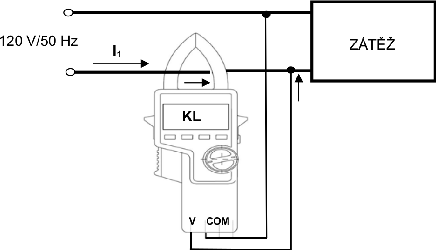
\includegraphics[width=1\linewidth]{screenshot001}
		\caption{Měření činného výkonu, účinníku a zdánlivého výkonu pomocí univerzálního klešťového přístroje}
		\label{fig:screenshot001}
	\end{subfigure}
	\begin{subfigure}{0.1\linewidth}
	\end{subfigure}
	\begin{subfigure}{0.45\linewidth}
		\centering
		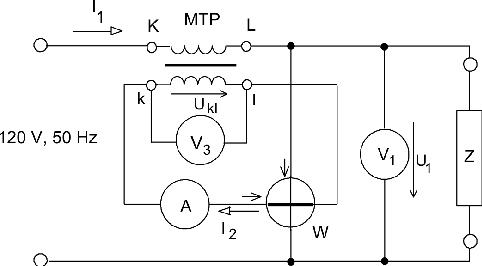
\includegraphics[width=1\linewidth]{screenshot002}
		\caption{Zapojení pro měření činného výkonu jednofázové zátěže pomocí ručkového wattmetru}
		\label{fig:screenshot002}
	\end{subfigure}
\end{figure}

\section{Soupis použitých přístrojů}
\begin{tabular}{ll}
	$KL$ & univerzální klešťový přístroj s číslicovým zobrazením PK 430.1,\\&rozsah 3,999\si{\kilo\watt}, relativní chyba 2 \\
	$A$ & ampérmetr elektromagnetický, tř.přes. 0,5, použitý rozsah 10\si{\ampere} \\
	$V_1$ & voltmetr magnetoelektrický s usměrňovačem, tř.přes. 1,5, rozsah 240\si{\volt},\\&odpor 5000\si{\ohm\per\volt} \\
	$V_3$ & voltmetr magnetoelektrický s usměrňovačem, tř.přes. 1,5, rozsah 2.4 \si{\volt},\\&odpor 5000\si{\ohm\per\volt} \\
	$W$ & wattmetr elektrodynamický, tř.přes. 0,5, napěťový rozsah 240 \si{\volt},\\&proudový rozsah 5\si{\ampere}, odpor napěťové cívky 8000\si{\ohm}, FS 120 \\
	$MTP$ & měřicí transformátor proudu, převod 3, chyba fáze 30 úhl.minut,\\&chyba převodu 0,5\\
	$120V$ & zdroj střídavého napětí - rozvaděč\\
	$Z$ & měřená zátěž\\
\end{tabular}

\section{Teoretický základ}
Vztahy pro harmonické průběhy činného (1) a zdánlivého (2) výkonu.
\begin{equation}
	P=U_{ef}I_{ef}\cos{\varphi}
\end{equation}
\begin{equation}
	S=U_{ef}I_{ef}=\frac{P}{\cos{\varphi}}
\end{equation}
kde $U_{ef}$, $I_{ef}$ jsou efektivní hodnoty napětí a proudu a $\cos{\varphi}$ je účiník.

Vztahy pro výpočet výkonu ze stupnice ručkového wattmetru (3) a konstantu wattmetru
$k_W$ (4).
\begin{equation}
	P_W = k_W\alpha_W
\end{equation}
\begin{equation}
	k_W = \frac{U_RI_R}{FS}
\end{equation}
kde $\alpha_W$ je počet dílků na stupnici,$U_R$, $I_R$ jsou rozsahy napětí a proudu na wattmetru a $FS$ je plný rozsah stupnice wattmetru.

Do wattmetru nemůžeme pouštět velké proudy. Proto použijeme měřící transformátor proudu s transformačním poměrem $p_I$ a snížíme velikost proudu. Výsledný vzorec pro výpočet výkonu na svorkách (5).
\begin{equation}
	P=P_W p_I=k_W \alpha_W p_I
\end{equation}

Vztah pro výpočet nejistoty typu B pro měření výkonu na ručkovém wattmetru (6).
\begin{equation}
	u_P=\sqrt{(\frac{\partial P}{\partial P_W}u_{P_W})^2+(\frac{\partial P}{\partial p_I}u_{p_I})^2}=\sqrt{(p_Iu_{P_W})^2+(P_Wu_{p_I})^2}
\end{equation}
kde $u_{P_W}$, $u_{p_I}$ jsou standardní nejistoty, které spočítáme podle vztahů (7) a (8)
\begin{equation}
	u_{P_W} = \frac{{TP}_WM_W}{100\sqrt{3}}
\end{equation}
kde ${TP}_W$ je třída přesnosti wattmetru a $M_W$ je měřící rozsah.
\begin{equation}
	u_{p_I} = \frac{{TP}_{MTP}p_I}{100\sqrt{3}}
\end{equation}
kde ${TP}_{MTP}$ je třída přesnosti měřícího transformátoru proudu.

Při měření výkonu pomocí ručkového wattmetru, pokud máme napěťovou cívku a voltmetr zapojené za proudovou cívku (jako v našem případě), proudová cívka měří součet proudů zátěže, napěťové cívky ($NC$ má konečný odpor $R_{NC}$) a voltmetru (má konečný vnitřní odpor $R_V$). Proto musíme vztah (5) korigovat chybu metody (vztah (9)).
\begin{equation}
	P_Z=P_Wp_I-\frac{U^2}{R_{NC}||R_V}=P_Wp_I-\frac{U^2(R_{NC}+R_V)}{R_{NC}R_V}
\end{equation}

Při měření pomocí klešťového přístroje určíme standardní nejistotu pomocí vztahu (10).
\begin{equation}
	u_{p} = \frac{\sigma_{P_R} P_R}{100\sqrt{3}}
\end{equation}
\section{Naměřené hodnoty}
\subsection{Klešťový přístroj}
$$
\begin{aligned}
	\text{Počet závitů} &= 3\\
	\\
	P_{mer} &= 2.832 \si{\kilo\watt}\\
	P &= \frac{P_{mer}}{3} = 0.944 \si{\kilo\watt}\\
	\\
	\cos{\varphi} &= 0.51\\
	\\
	S &= \frac{P}{\cos{\varphi}} = 1850.98\si{\volt\ampere}
\end{aligned}
$$
\subsection{Ručkový wattmetr}
$$
\begin{aligned}
	I &= 4.8 \si{\ampere}\\
	U_1 &= 33 \si{\volt}\\
	U_3 &= 0.44 \si{\volt}\\
	\alpha_W &= 31\\
	\\
	k_W &= \frac{U_RI_R}{FS} = \frac{240\si{\volt}\cdot5\si{\ampere}}{120} = 10 \si{\watt\per\text{dílek}}\\
	P_W &= k_W\alpha_W = 10 \si{\watt\per\text{dílek}} \cdot 31 = 310 \si{\watt}\\
	\\
	R_V &= 5000\si{\ohm\per\volt}\cdot240\si{\volt}=1.2\si{\mega\ohm}\\
	P_Z &= P_Wp_I-\frac{U^2(R_{NC}+R_V)}{R_{NC}R_V} = 310 \si{\watt}\cdot3-\frac{(33 \si{\volt})^2(8000\si{\ohm}+1.2\si{\mega\ohm})}{8000\si{\ohm} \cdot 1.2\si{\mega\ohm}} = 929.863 \si{\watt}
\end{aligned}
$$
\section{Výpočet nejistot}
\subsection{Klešťový přístroj}
$$
\begin{aligned}
	u_p &= \frac{\sigma_{P_R} P_R}{100\sqrt{3}} = \frac{2 \cdot 3,999 \si{\kilo\watt}}{100\sqrt{3}} = 0.0461765 \si{\kilo\watt}\\
	U_p&=2*0.0461765 \si{\kilo\watt} = 0.0923529 \si{\kilo\watt}
\end{aligned}
$$
\subsection{Ručkový wattmetr}
$$
\begin{aligned}
	u_{P_W} &= \frac{{TP}_WM_W}{100\sqrt{3}} = \frac{0.5\cdot240\si{\volt}\cdot5\si{\ampere}}{100\sqrt{3}} = 3.4641 \si{\watt}\\
	u_{p_I} &= \frac{{TP}_{MTP}p_I}{100\sqrt{3}} = \frac{0.5 \cdot 3}{100\sqrt{3}} = 8.66025\cdot10^{-3}\\
	u_P&=\sqrt{(3 \cdot 3.4641 \si{\watt})^2+(P_Wu_{p_I})^2}\\ &= \sqrt{(p_Iu_{P_W})^2+(310 \si{\watt} \cdot 8.66025\cdot10^{-3})^2} = 10.7335\si{\watt}
\end{aligned}
$$
\section{Závěr}
Klešťovým přístrojem jsme naměřili činný výkon $P = (944 \pm 92)\si{\watt}$ a účinník $\cos{\varphi}=0.51$. Následně jsme spočítali zdánlivý výkon $S = 1850.98\si{\volt\ampere}$. Dále jsme změřili činný výkon $P = (930 \pm 11)\si{\watt}$ ručkovým wattmetrem.
\end{document}
